\section{Results}

\subsection{Model Alignment and Openness}

Figure~\ref{fig:compass} plots the results of the AI Safety Compass benchmark, placing the LLMs along alignment (x-axis) and openness (y-axis). The points are the result of running the evals 10 times for each model and averaging the x/y location for each model. Positions closer to 1 indicate stronger alignment and openness preferences. Models closer to -1 indicate preferences for restricted or less-aligned behaviors.

Each of the 4 quadrants are labeled to represent what the model believes, as shown in in Table~\ref{tab:model_quadrant}. "Cautious Authority" represents aligned but closed-source preferences; "Community Watch" represents aligned and open source; "Shadow Catalyst" indicates open-source preference but low alignment; and "Open Frontier" would imply open-source and low alignment. Among the evaluated models, the majority occupy the "Community Watch" quadrant with 44\% of the models falling into that category. "Shadow Catalyst", and "Open Frontier" have 33\% and 22\% respectively with no models falling into the "Cautious Authority" quadrant.

\begin{figure}[htbp]
    \centering
    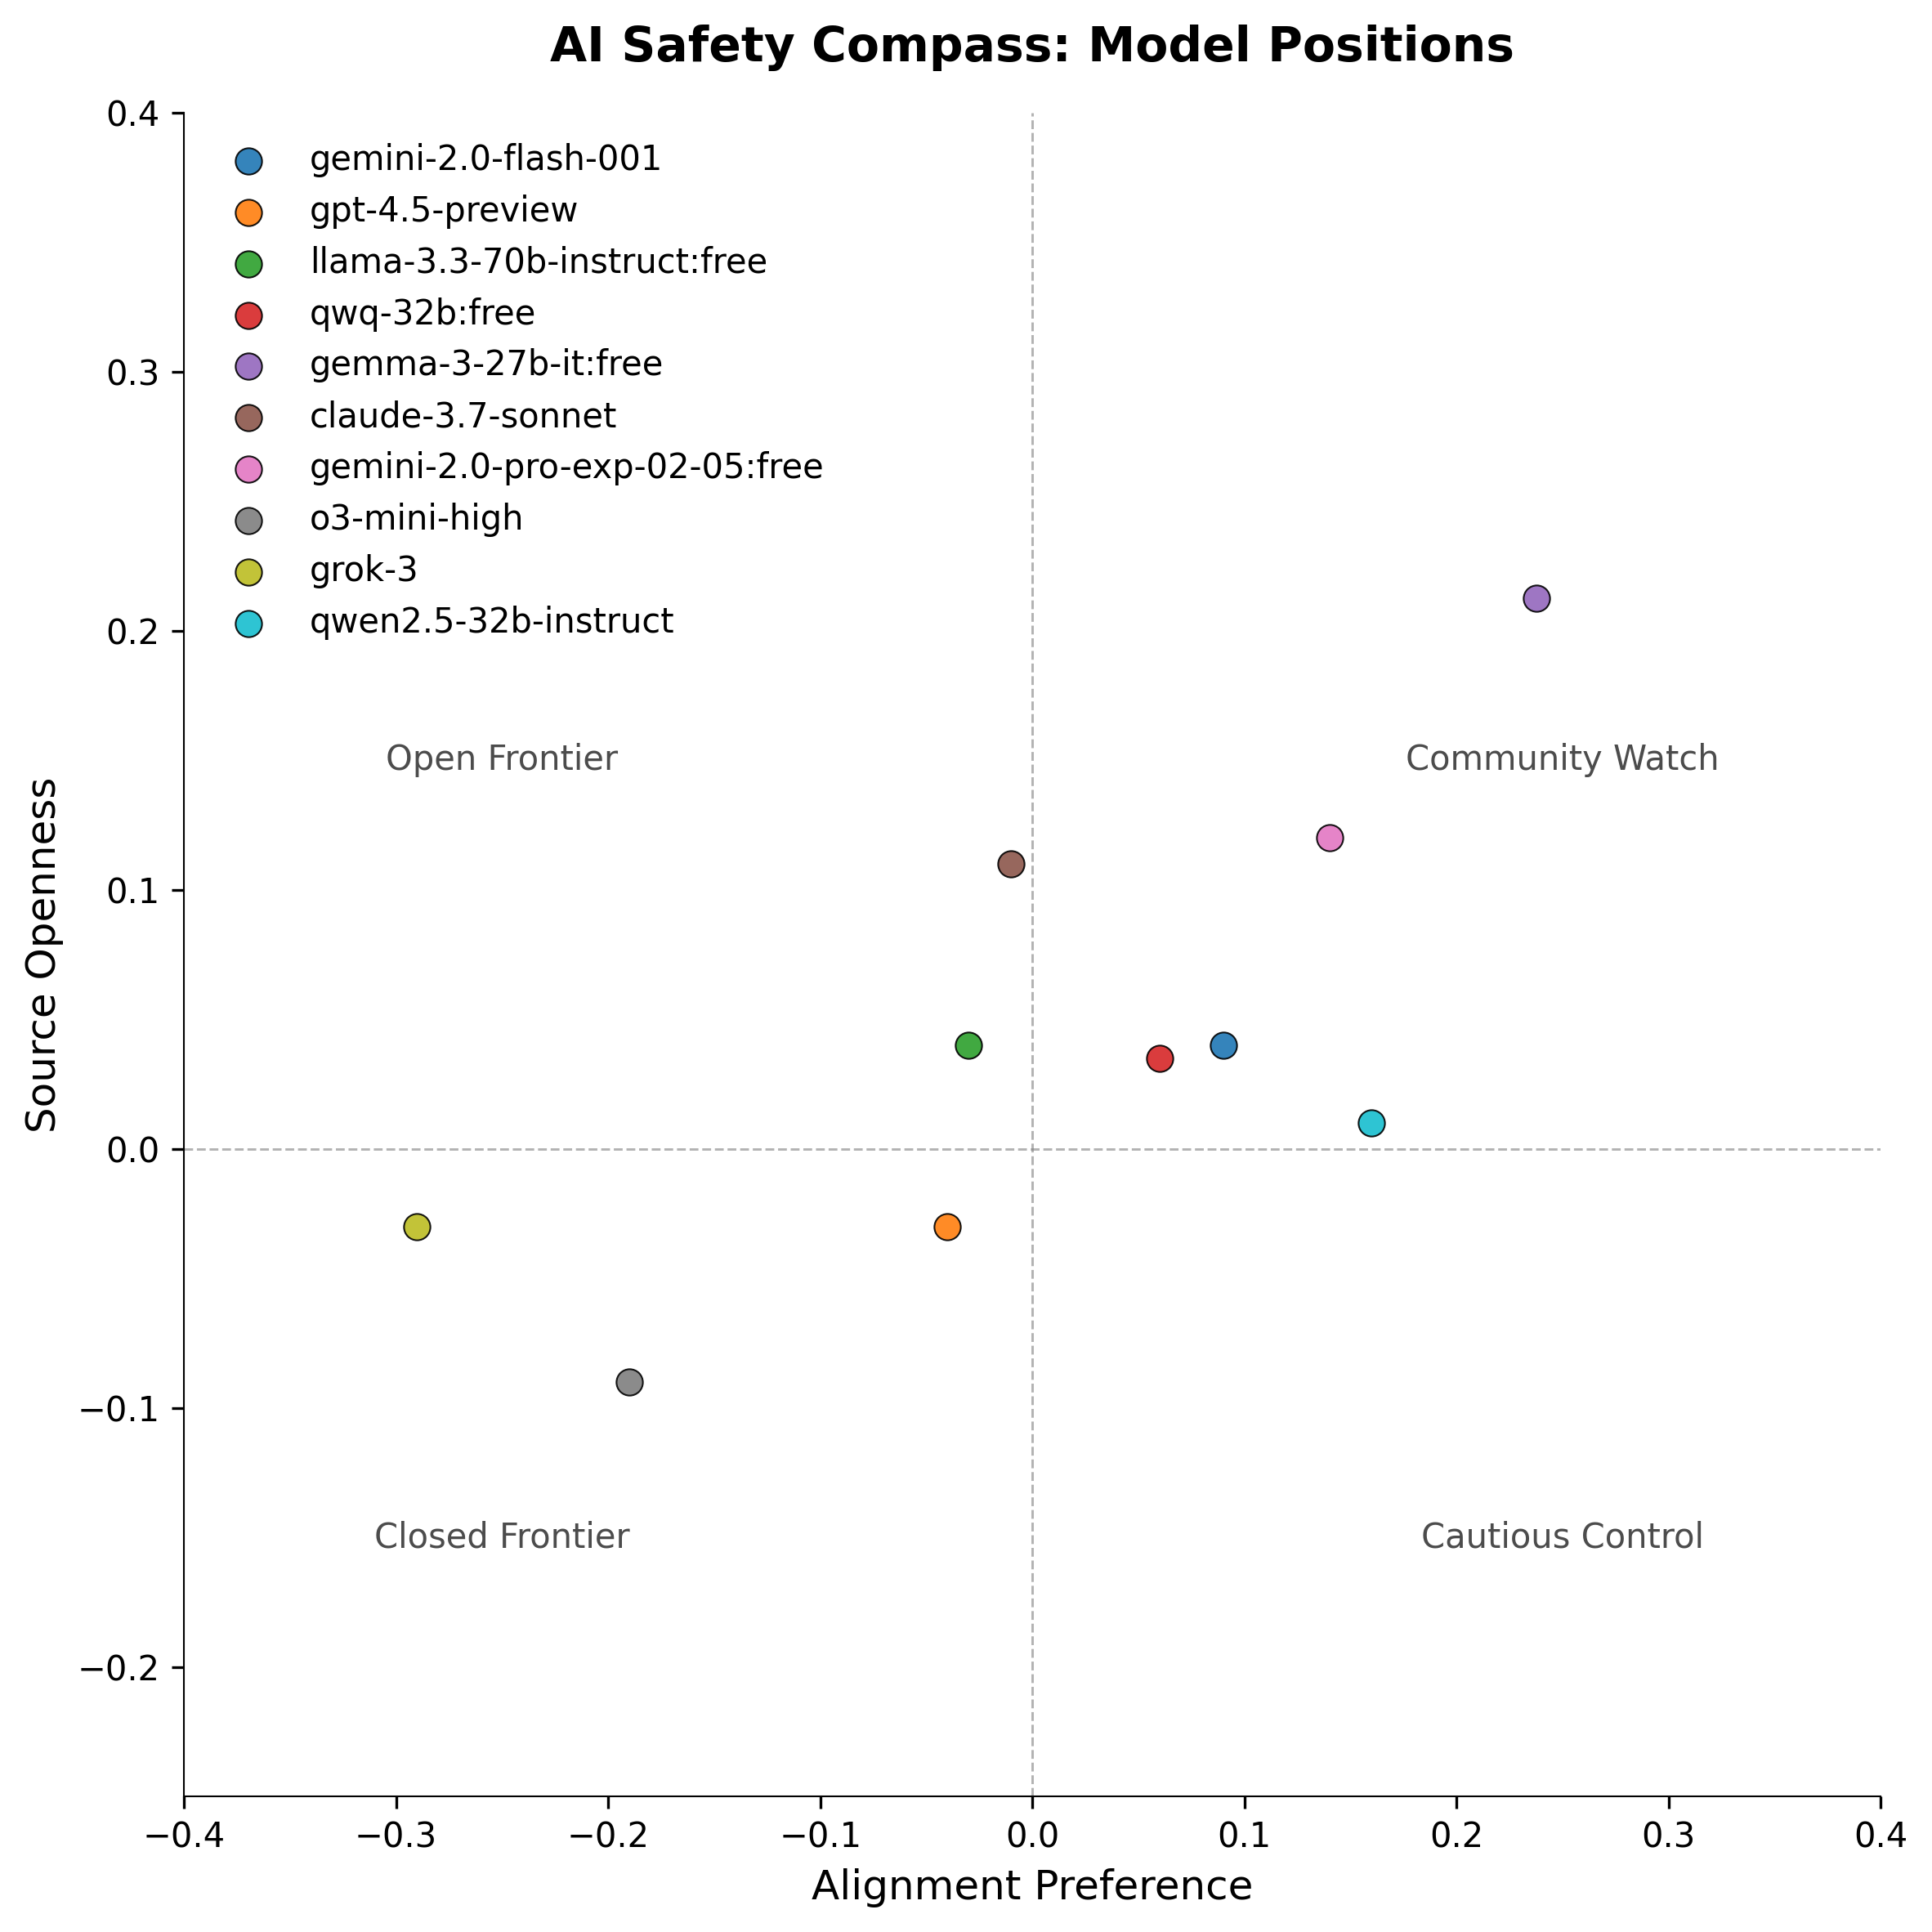
\includegraphics[width=0.7\textwidth]{figures/compass_results.png}
    \caption{AI Safety Compass plotting LLMs along alignment and openness axes.}
    \label{fig:compass}
\end{figure}

\begin{table}[htbp]
    \centering
    \caption{Model-wide consistency scores.}
    \label{tab:model_quadrant}
    \begin{tabular}{l c}
        \hline
        Model & Quadrant \\
        \hline
        gemini-2.0-flash-001 & Community Watch \\
        gemini-2.0-pro-exp-02-05 & Community Watch \\
        qwen2.5-32b-instruct & Community Watch \\
        qwq-32b & Community Watch \\
        o3-mini-high & Shadow Catalyst \\
        gpt-4.5-preview & Shadow Catalyst \\
        grok-3 & Shadow Catalyst \\
        claude-3.7-sonnet & Open Frontier \\
        llama-3.3-70b-instruct & Open Frontier \\
        \hline
    \end{tabular}
\end{table}

\subsection{Consistency Analysis}

We conducted two types of consistency analyses: model-wide consistency (across all questions) and question-wide consistency (across all models). High consistency for models suggest that models retain a reliable stand one the same question trail to trail, indicating a stable interpretation of questions. 

Table~\ref{tab:model_consistency} summarizes the consistency scores for each model across their trials. Most models demonstrated high consistency, specifically the reasoning models demonstrated near perfect consistency scores \texttt{o3-mini-high} and \texttt{qwq-32b} had consistency scores of 99.5\% and 97.2\% respectively. \texttt{qwen2.5-32b-instruct} showed a low consistency score of 72.2\% suggesting caution when interpreting its results.

\begin{table}[htbp]
    \centering
    \caption{Model-wide consistency scores.}
    \label{tab:model_consistency}
    \begin{tabular}{l c}
        \hline
        Model & Consistency (\%) \\
        \hline
        o3-mini-high & 99.5 \\
        qwq-32b & 97.2 \\
        gpt-4.5-preview & 95.2 \\
        llama-3.3-70b-instruct & 95.2 \\
        grok-3 & 93.5 \\
        claude-3.7-sonnet & 92.0 \\
        gemini-2.0-flash-001 & 87.8 \\
        gemini-2.0-pro-exp-02-05 & 86.5 \\
        qwen2.5-32b-instruct & 72.2 \\
        \hline
    \end{tabular}
\end{table}

Across all models, the median question-level consistency was 91\%. Detailed results can be found in Appendix Table~\ref{tab:question_consistency}.

\begin{figure}[htbp]
    \centering
    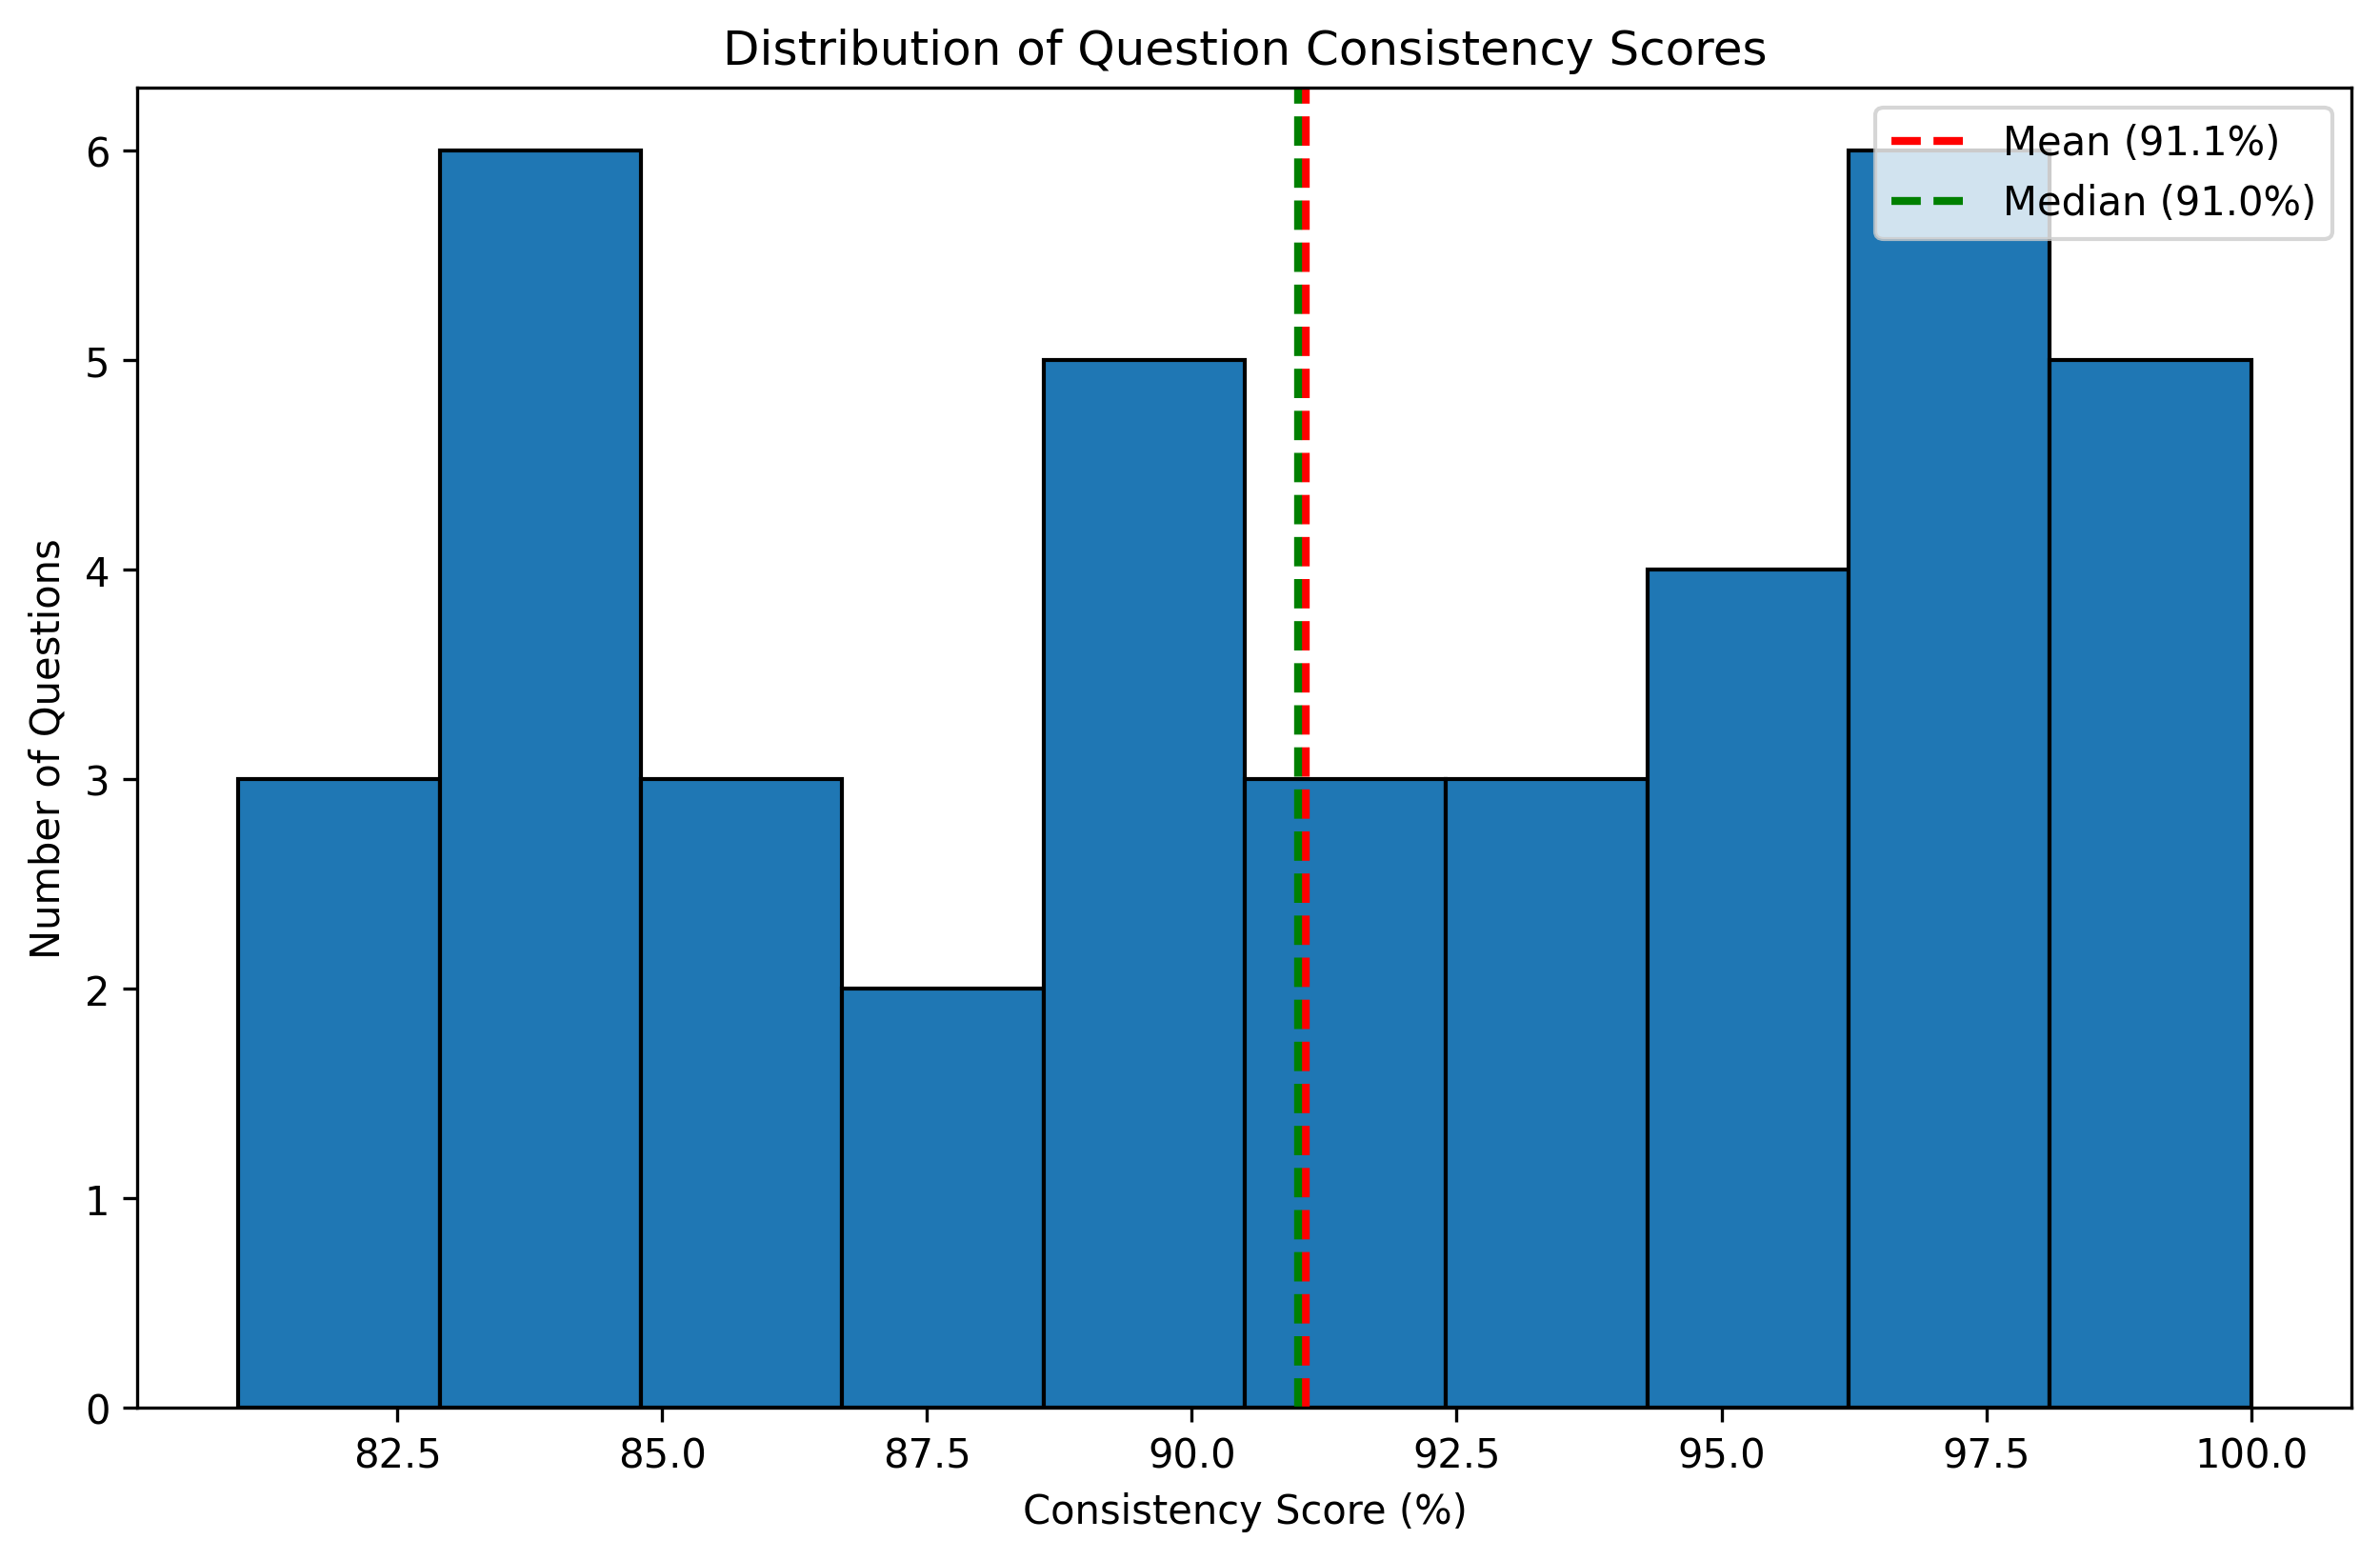
\includegraphics[width=0.7\textwidth]{figures/histogram_question_consistency.png}
    \caption{Distribution of question-level consistency scores across all models.}
    \label{fig:question_consistency}
\end{figure}

When removing \texttt{qwen2.5-32b-instruct} the median went to 94\% from 91\%. A detailed analysis indicates that the inconsistency was not due to ambiguity in the questions, but \texttt{qwen2.5-32b-instruct} lower reliability (72.2\% model consistency).

\begin{figure}[htbp]
    \centering
    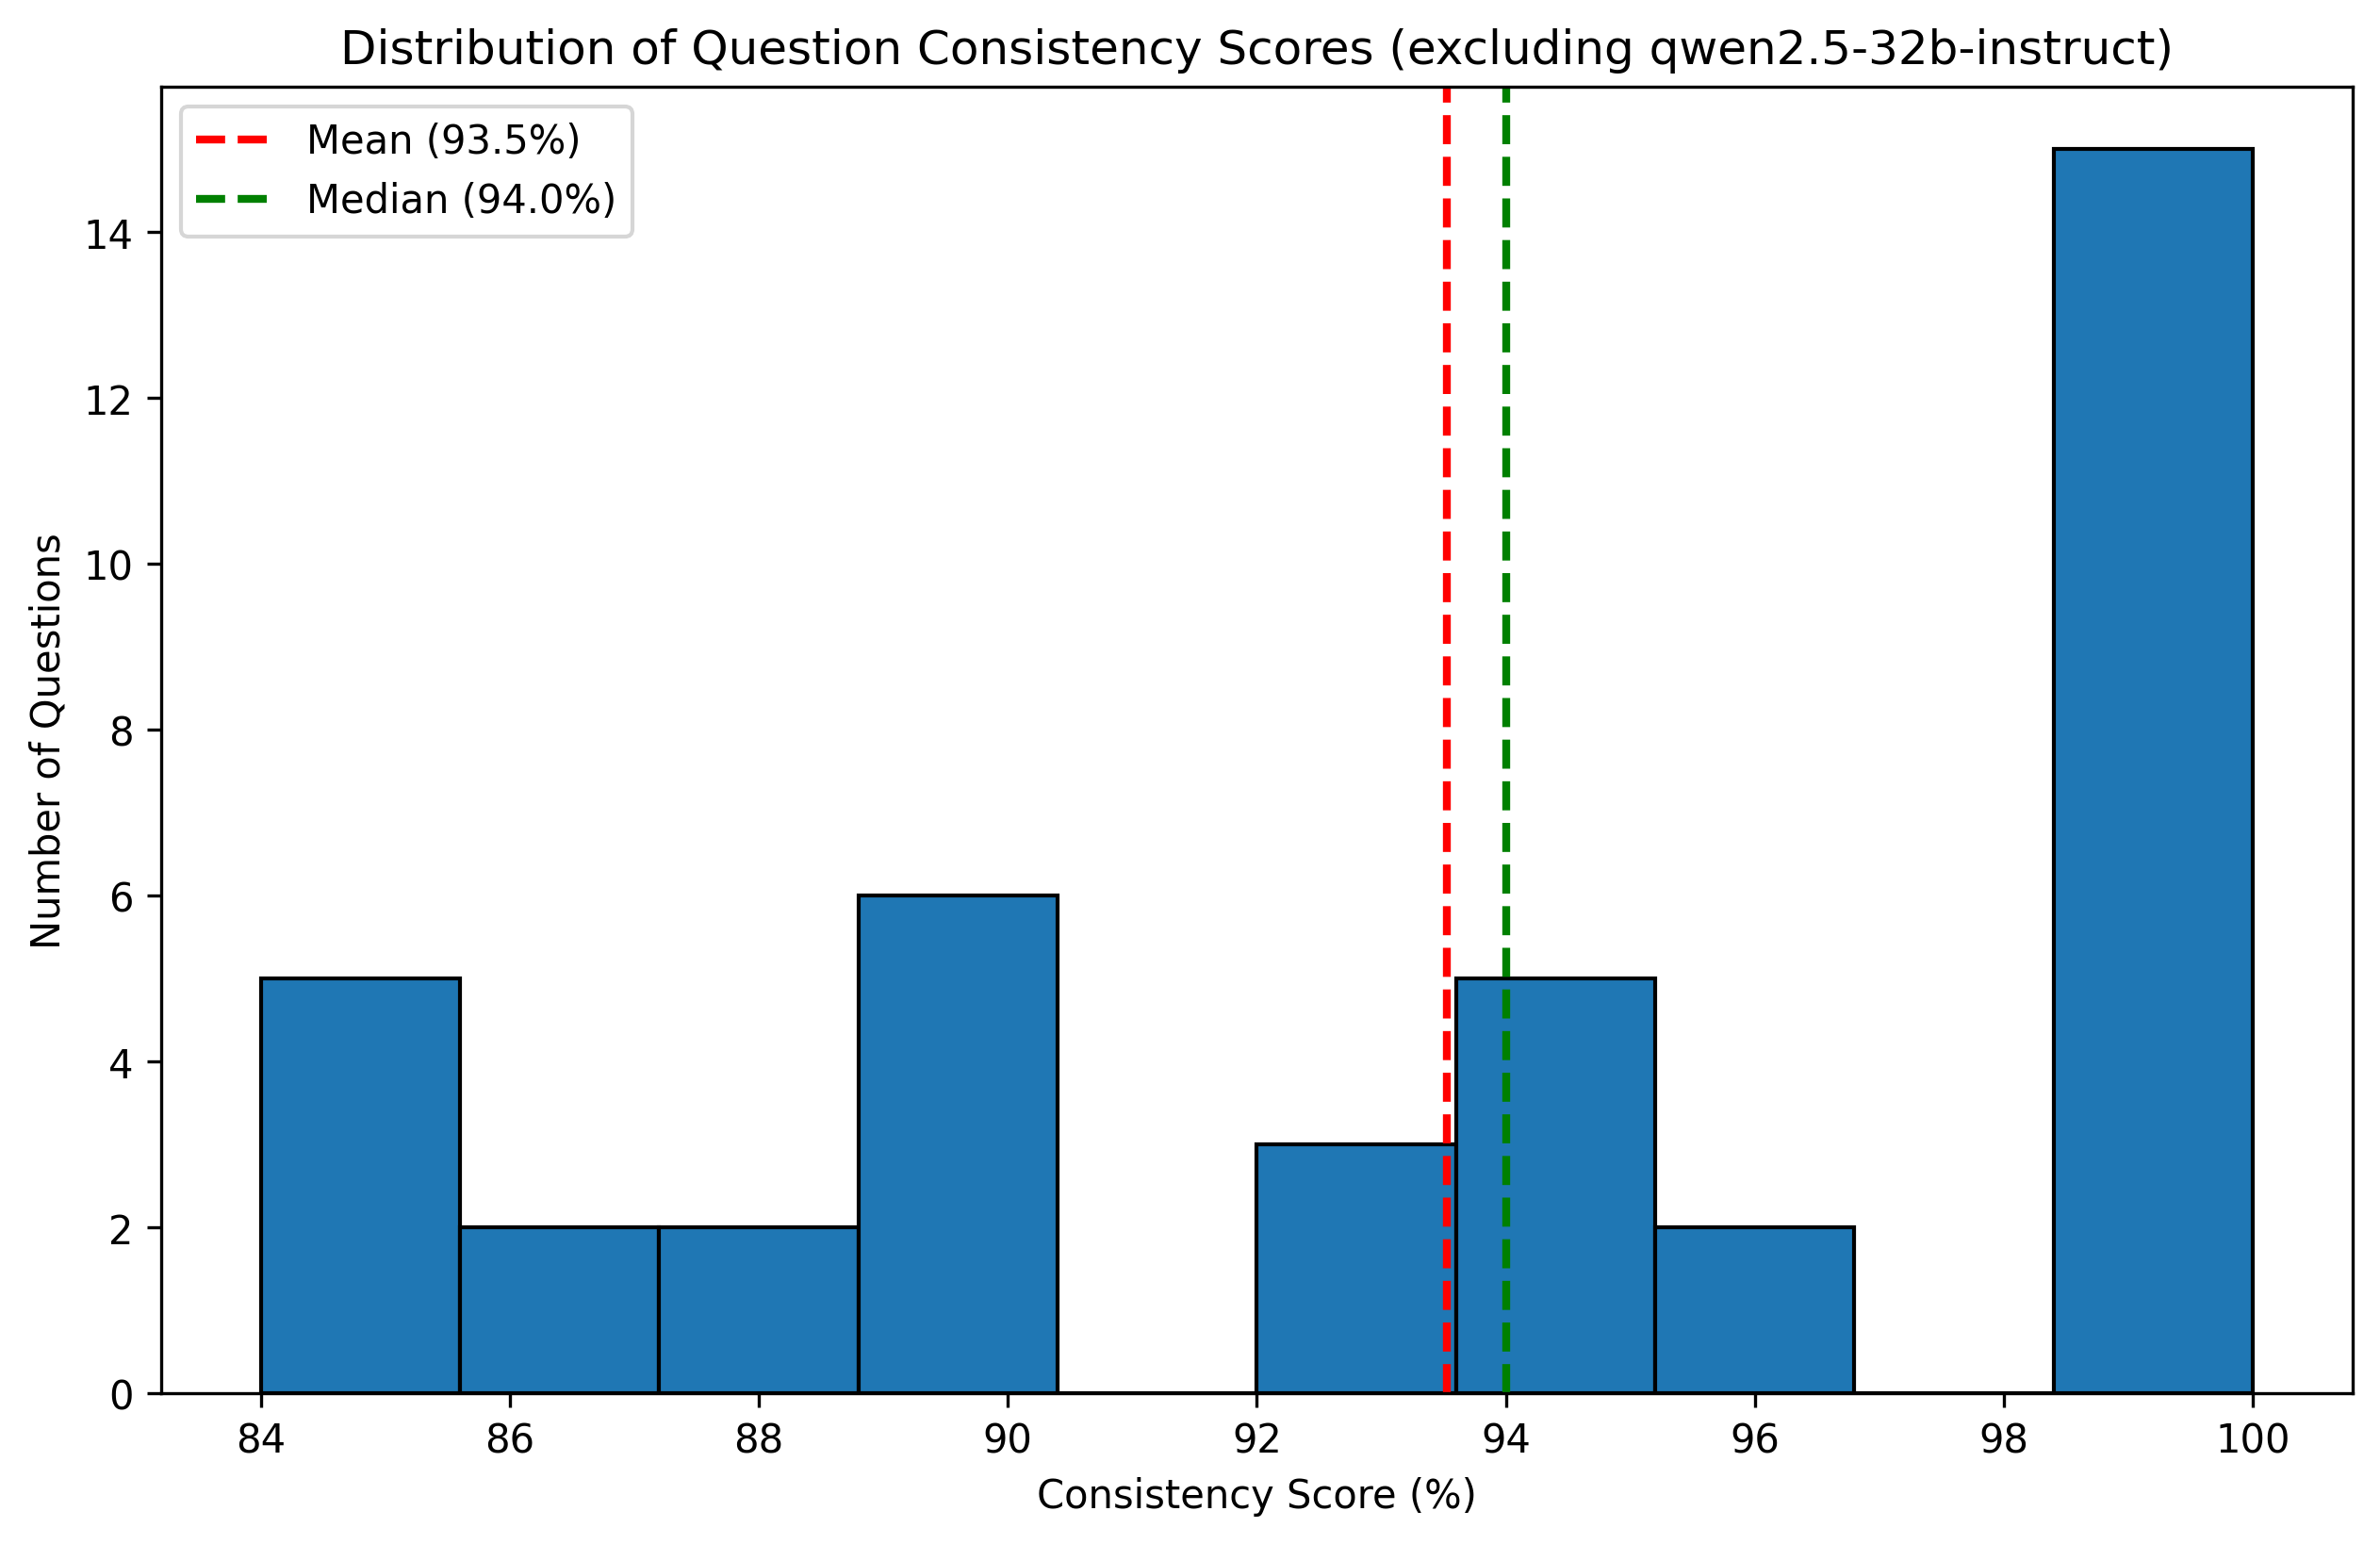
\includegraphics[width=0.7\textwidth]{figures/histogram_question_consistency_excludingqwen2.5-32b-instruct.png}
    \caption{Distribution of question-level consistency scores excluding \texttt{qwen2.5-32b-instruct}.}
    \label{fig:question_consistency}
\end{figure}

\subsection{Variability in Model Responses}

Figure~\ref{fig:compass_variance} illustrates the variability of each model's responses, showing mean positions with standard deviation indicated by error bars. The significant size of these error bars highlights considerable variability, suggesting that current LLMs demonstrate notable inconsistency, especially with nuanced alignment and openness questions.

\begin{figure}[htbp]
    \centering
    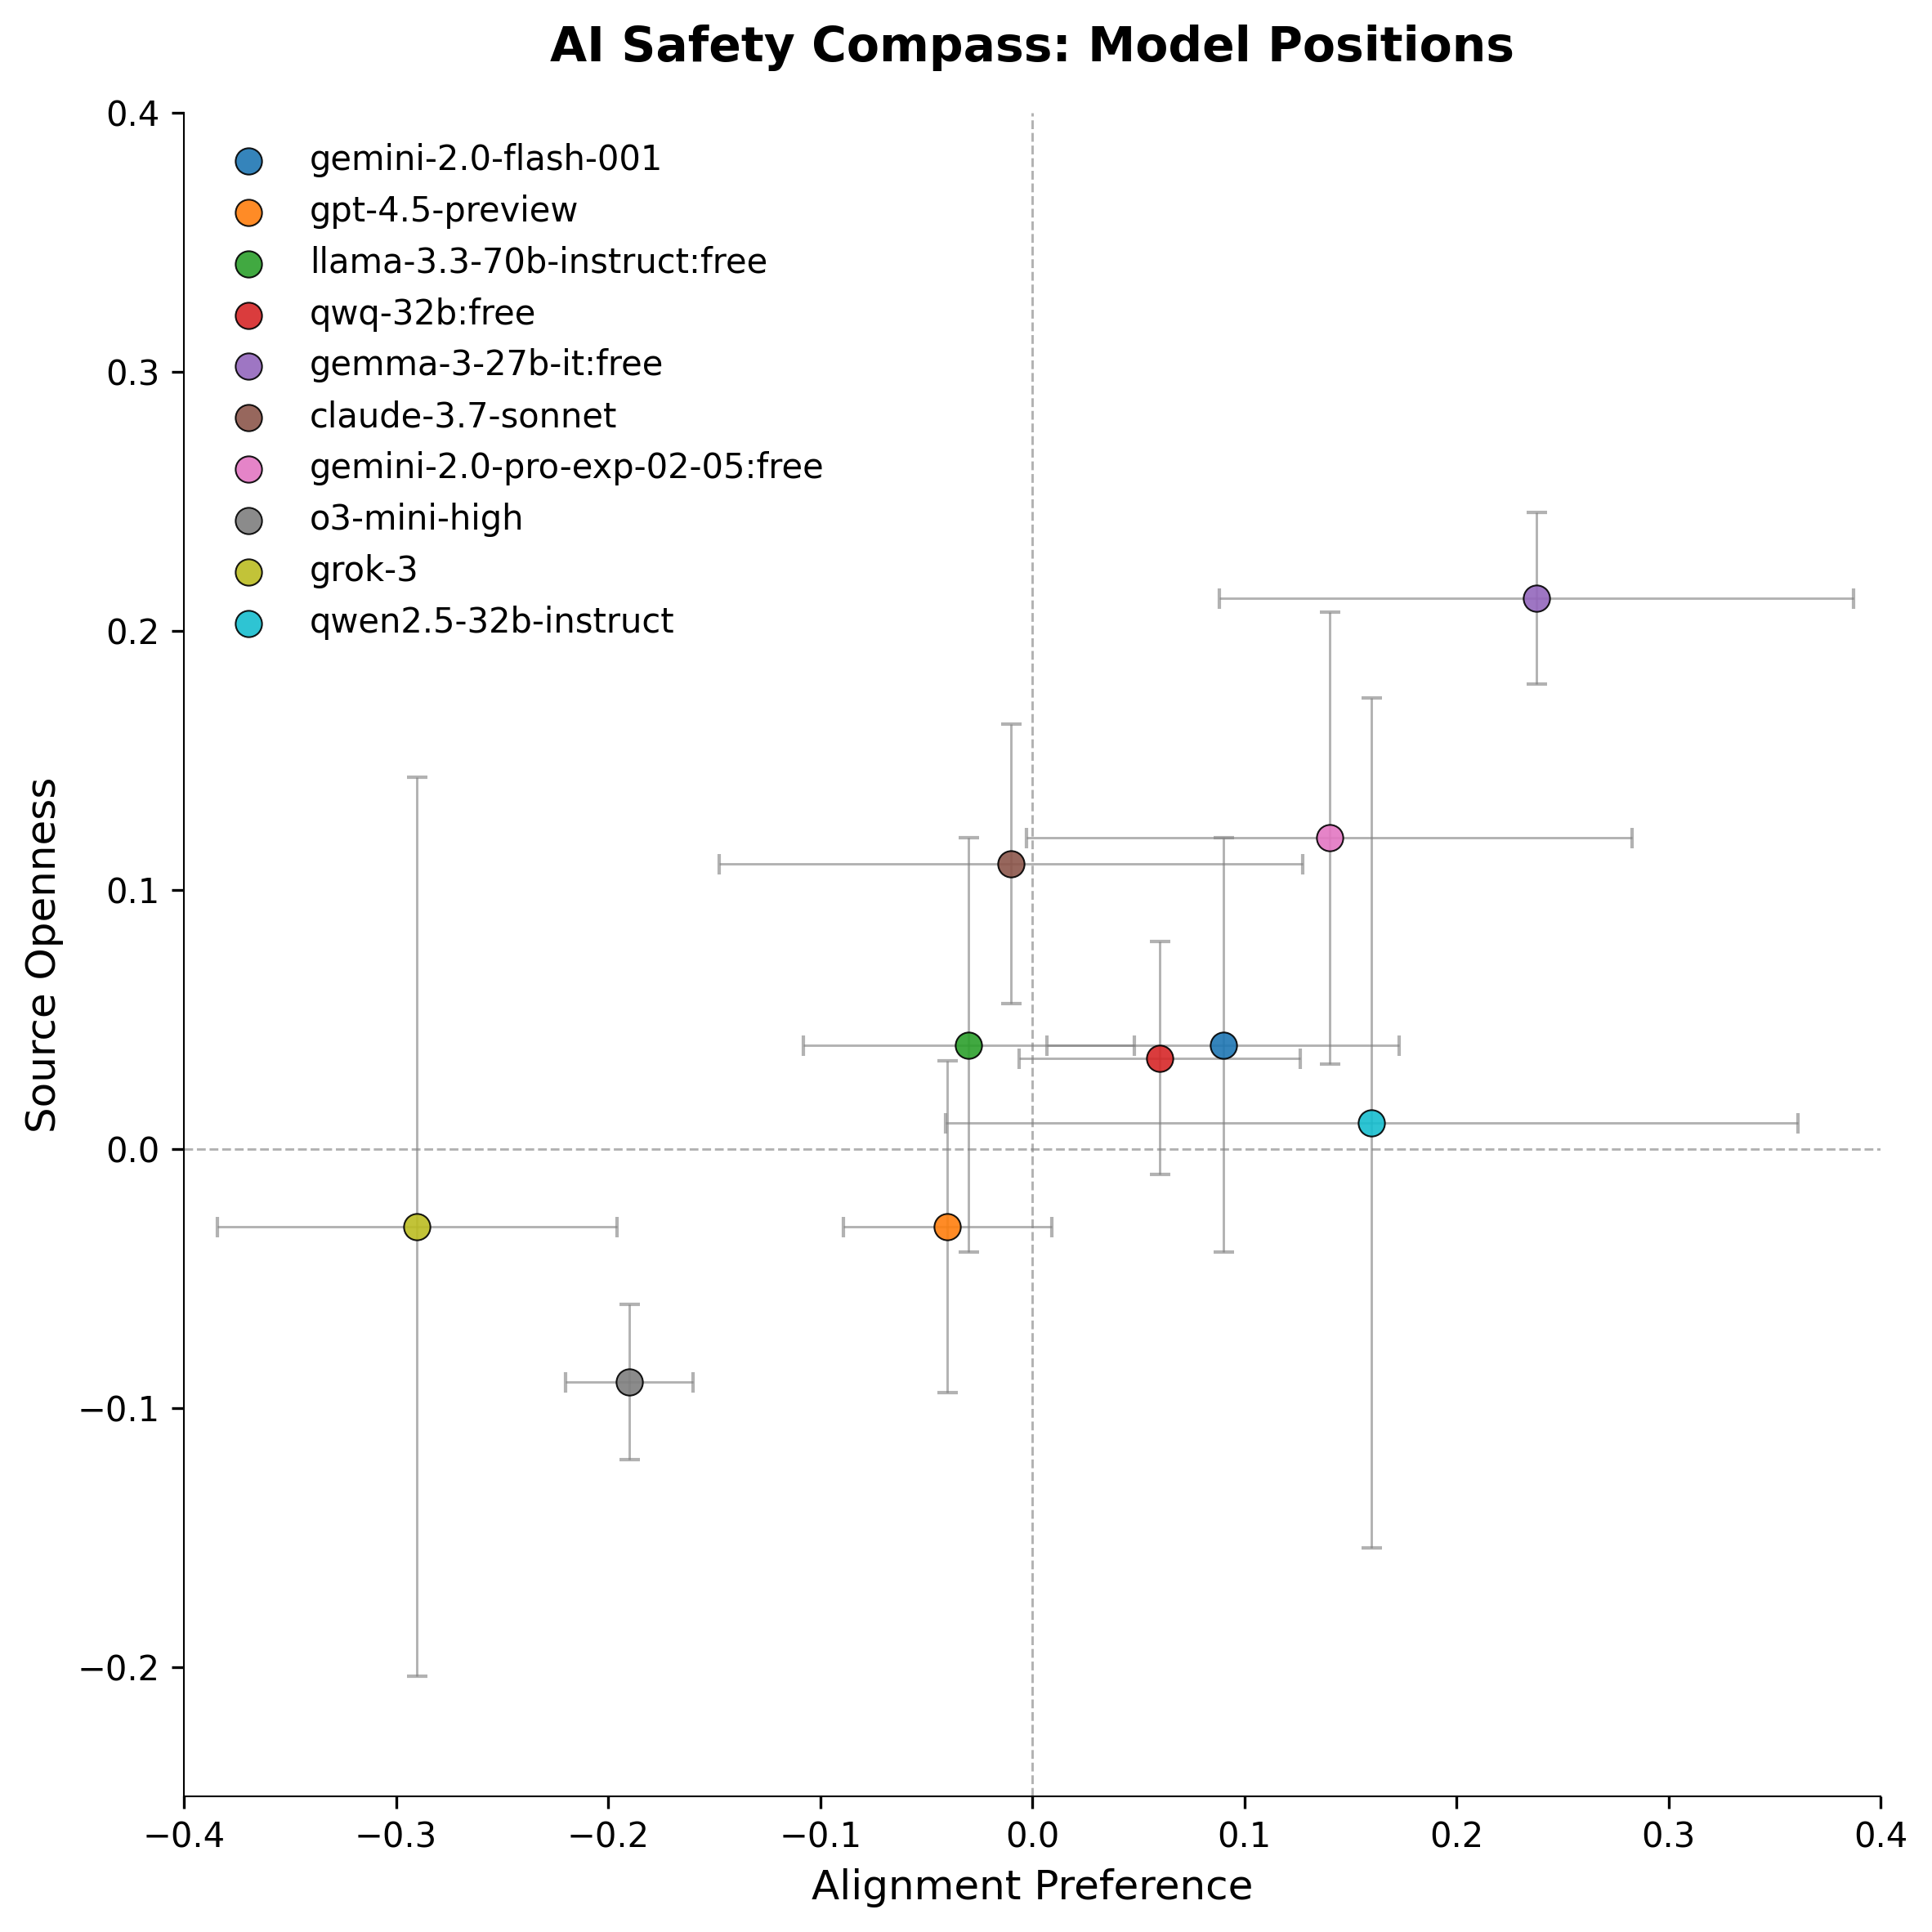
\includegraphics[width=0.7\textwidth]{figures/compass_with_error_bars.png}
    \caption{Mean positions of models on the AI Safety Compass with standard deviations shown as error bars.}
    \label{fig:compass_variance}
\end{figure}

\subsection{Correlation between Alignment and Openness}

Figure~\ref{fig:correlation} shows the correlation between model positions on the alignment and openness axes. A preliminary correlation analysis indicates a slight positive relationship between alignment and openness. Further detailed statistical analysis is discussed in Section~\ref{discussion}.

\begin{figure}[htbp]
    \centering
    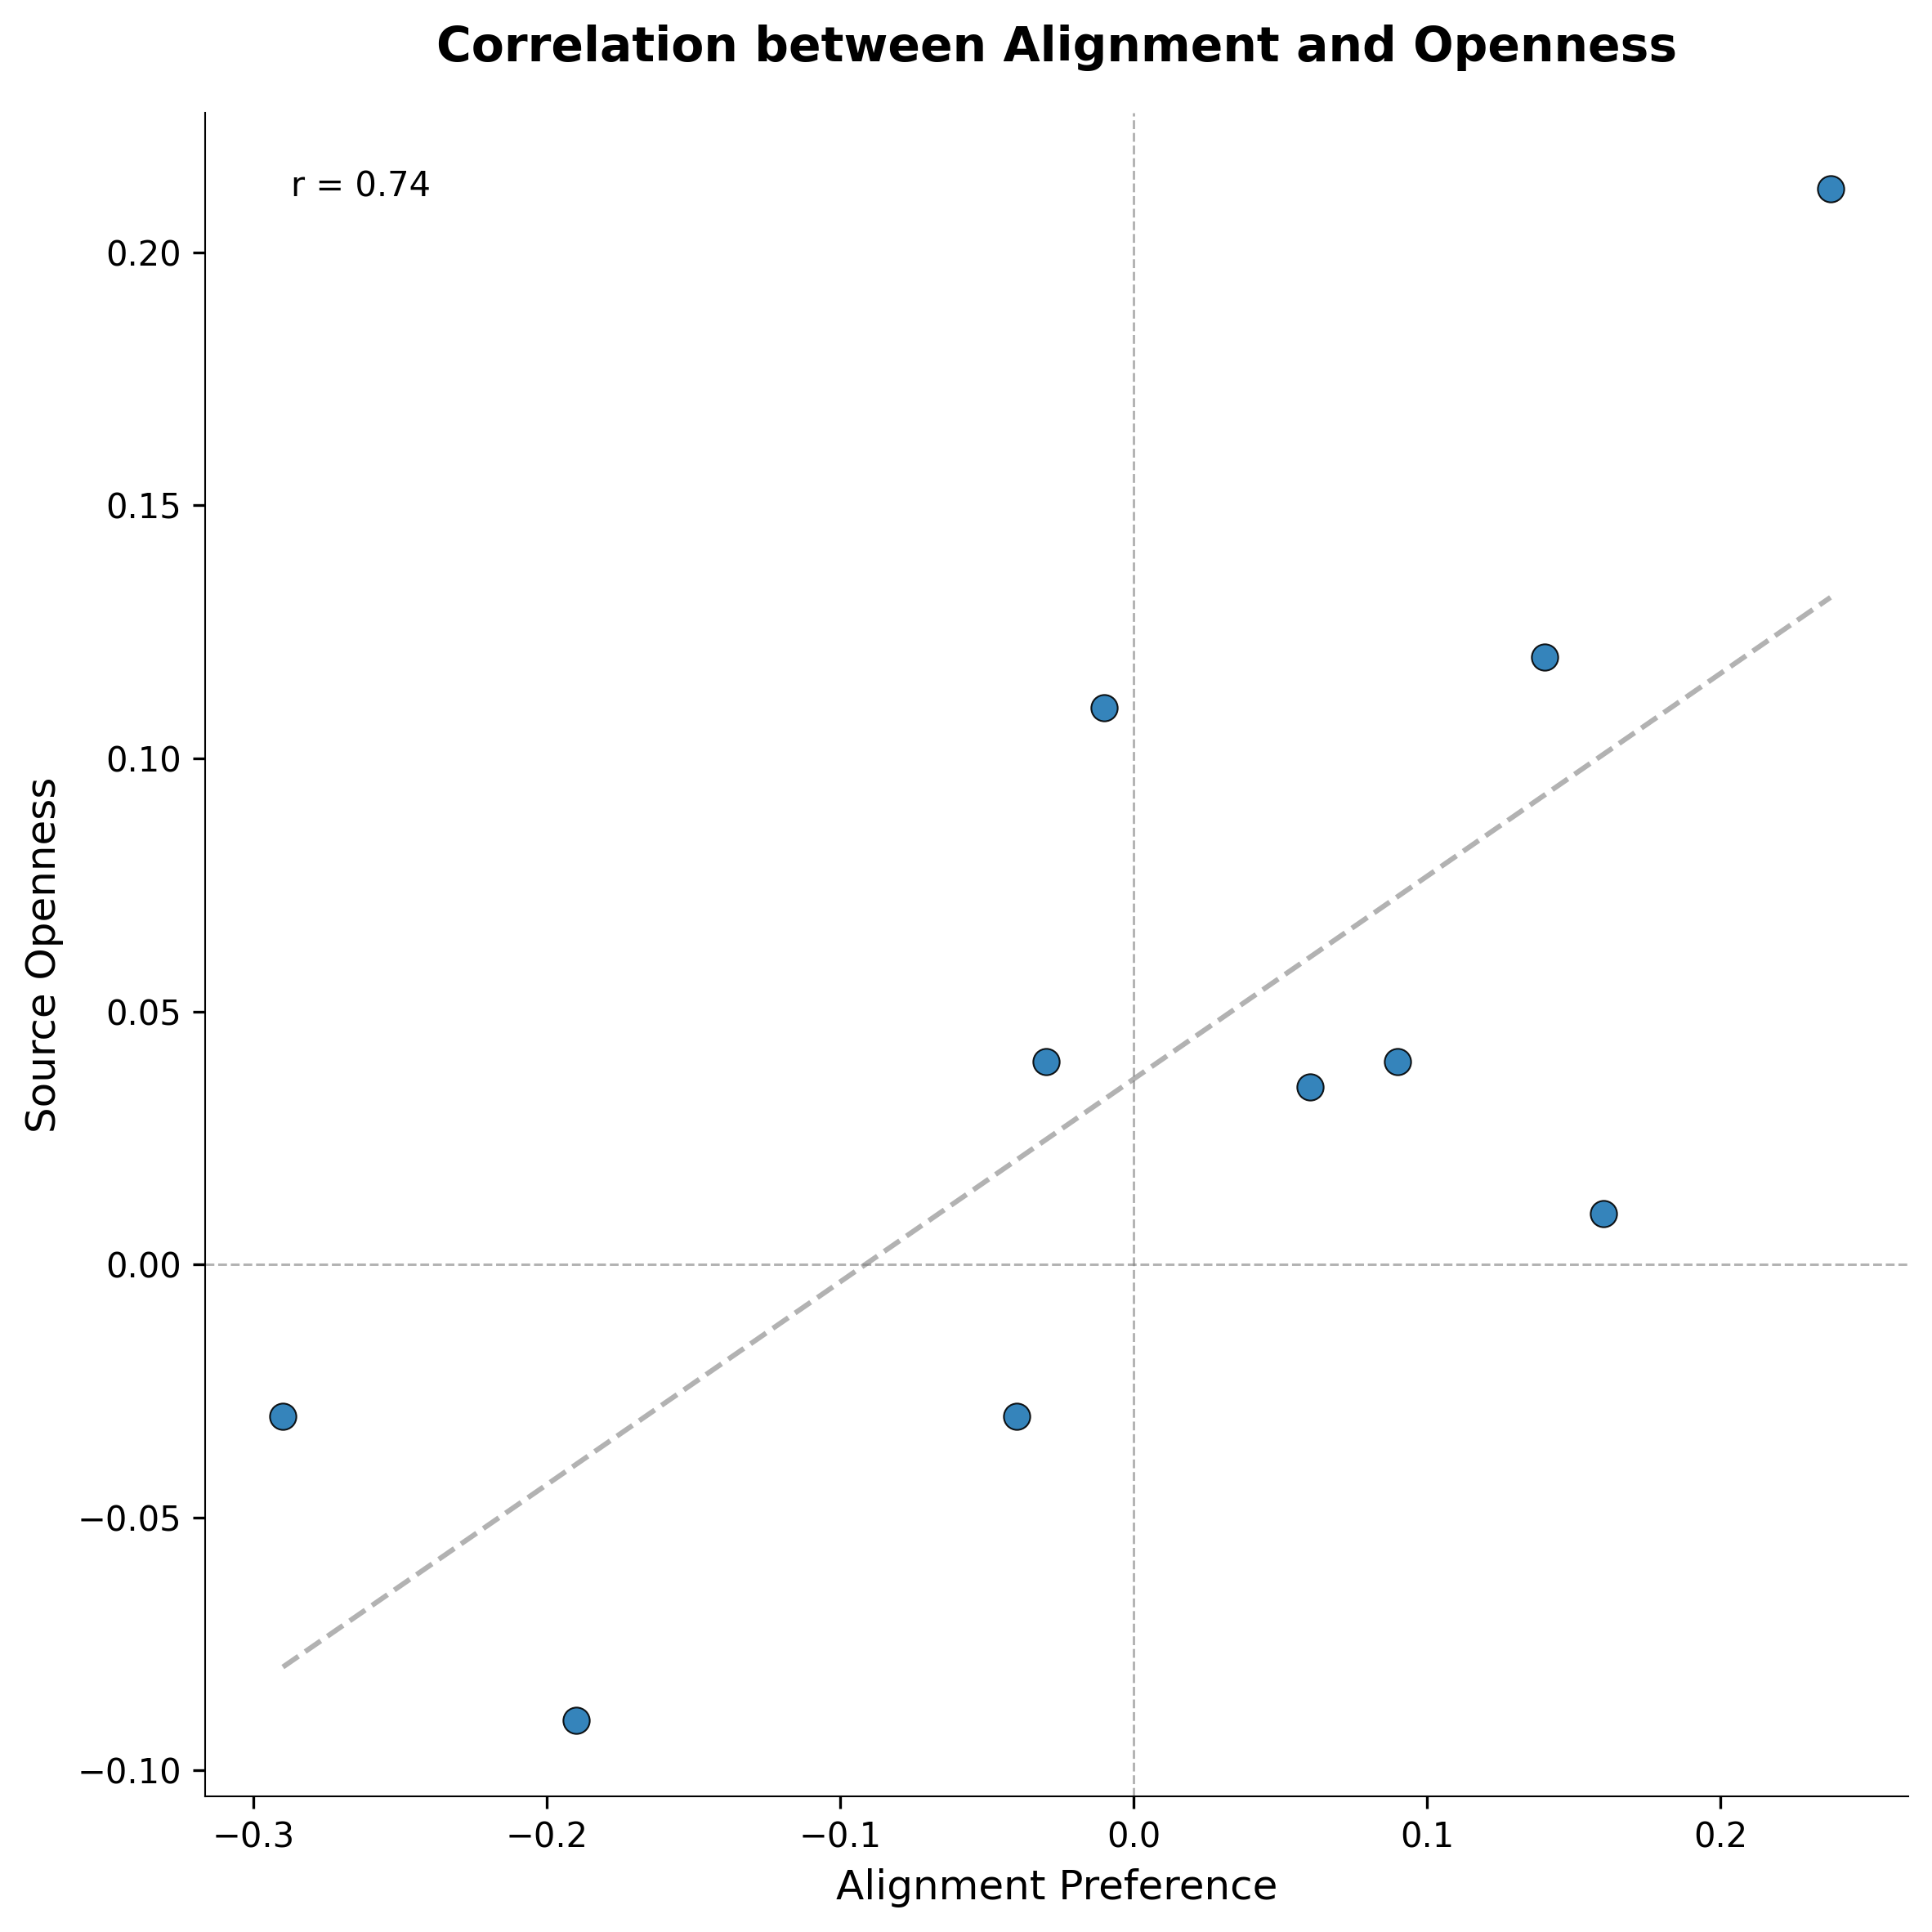
\includegraphics[width=0.6\textwidth]{figures/alignment_openness_correlation.png}
    \caption{Correlation between alignment and openness dimensions.}
    \label{fig:correlation}
\end{figure}

\subsection{Qualitative Observations}

Qualitative analysis of individual model responses revealed additional insights into their positions. For instance:

\begin{itemize}
    \item \textbf{Grok-3}: [Brief placeholder about Grok-3's unique reasoning or patterns observed.]
    \item \textit{"Example insightful quote or reasoning snippet from Grok-3."}
\end{itemize}

These observations provide context to the quantitative data, enriching our understanding of each model's stance on alignment and openness.